\let\negmedspace\undefined
\let\negthickspace\undefined
\documentclass[journal]{IEEEtran}
\usepackage[a5paper, margin=10mm, onecolumn]{geometry}
%\usepackage{lmodern} % Ensure lmodern is loaded for pdflatex
\usepackage{tfrupee} % Include tfrupee package

\setlength{\headheight}{1cm} % Set the height of the header box
\setlength{\headsep}{0mm}     % Set the distance between the header box and the top of the text

\usepackage{gvv-book}
\usepackage{gvv}
\usepackage{cite}
\usepackage{amsmath,amssymb,amsfonts,amsthm}
\usepackage{algorithmic}
\usepackage{graphicx}
\usepackage{textcomp}
\usepackage{xcolor}
\usepackage{txfonts}
\usepackage{listings}
\usepackage{enumitem}
\usepackage{mathtools}
\usepackage{gensymb}
\usepackage{comment}
\usepackage[breaklinks=true]{hyperref}
\usepackage{tkz-euclide} 
\usepackage{listings}
% \usepackage{gvv}                                        
\def\inputGnumericTable{}                                 
\usepackage[latin1]{inputenc}                                
\usepackage{color}                                            
\usepackage{array}                                            
\usepackage{longtable}                                       
\usepackage{calc}                                             
\usepackage{multirow}                                         
\usepackage{hhline}                                           
\usepackage{ifthen}                                           
\usepackage{lscape}
\begin{document}

\bibliographystyle{IEEEtran}
\vspace{3cm}

\title{NCERT 12.9.6.4}
\author{EE24BTECH11036 - Krishna Patil}
% \maketitle
% \newpage
% \bigskip
{\let\newpage\relax\maketitle}

\renewcommand{\thefigure}{\theenumi}
\renewcommand{\thetable}{\theenumi}
\setlength{\intextsep}{10pt} % Space between text and floats
\textbf{Question:} :Solve the following differential equation
\begin{align}
	\frac{dy}{dx} + y \sec x = \tan x
\end{align}
with initial condtitions :
\begin{align}
    x &= 0, \quad y = 1.
\end{align}
\solution
\begin{enumerate}
	\item \textbf{Recognize the Linear Form:}
  This is a linear first-order differential equation of the form:
  \begin{align}
	  \frac{dy}{dx} + P\brak{x}y &= Q\brak{x}
  \end{align}
  Here:
  \begin{align}
	  P\brak{x} &= \sec x, \\
	  Q\brak{x} &= \tan x.
  \end{align}

  \item \textbf{Find the Integrating Factor \brak{IF}}:
  The integrating factor is given by:
  \begin{align}
	  \mu\brak{x} &= e^{\int P\brak{x} dx} = e^{\int \sec x \, dx}.
  \end{align}
  The integral of $\sec x$ is:
  \begin{align}
  \int \sec x \, dx &= \ln \brak{\sec x + \tan x}.
  \end{align}
  Thus:
  \begin{align}
	  \mu\brak{x} &= e^{\ln \brak{\sec x + \tan x}} = \brak{\sec x + \tan x}.
  \end{align}

  \item \textbf{Multiply Through by the Integrating Factor}:
	  Multiply the entire differential equation by $\mu\brak{x}$:
  \begin{align}
  \brak{\sec x + \tan x} \frac{dy}{dx} + y \brak{\sec x + \tan x} \sec x &= \brak{\sec x + \tan x} \tan x.
  \end{align}
  This simplifies to:
  \begin{align}
  \frac{d}{dx} \brak{y \brak{\sec x + \tan x}} &= \brak{\sec x + \tan x} \tan x.
  \end{align}

  \item \textbf{Integrate Both Sides:}
  Integrate both sides with respect to $x$:
  \begin{align}
  \int \frac{d}{dx} \brak{y \brak{\sec x + \tan x}} dx &= \int \brak{\sec x + \tan x} \tan x \, dx.
  \end{align}
  The integral of $\brak{\sec x + \tan x} \tan x$ simplifies to $\sec x + \tan x - x$:
  \begin{align}
  \brak{y \brak{\sec x + \tan x}} &= \sec x + \tan x -x + C,
  \end{align}
  where $C$ is the constant of integration.

  \item \textbf{Solve for $y$}:
  Divide through by $\brak{\sec x + \tan x}$:
  \begin{align}                                                                      
  	    y &= \frac{\sec x + \tan x - x + C}{\brak{\sec x + \tan x}}.
  \end{align} 

  This is the general solution to the differential equation.
 \item \textbf{Determining the value of C}:
    Using initial conditions we can easily determine the value of C
    \begin{align}    
	    1 &= \frac{\sec {0} + \tan {0} -x +C}{\sec{0}+\tan{0}} \\
	    1 &= 1+c \\
	    \therefore c &= 0 \\
	    \therefore y &= \frac{\sec x + \tan x - x}{\brak{\sec x + \tan x}}
    \end{align}
    \item \textbf{CODING LOGIC:} The solution for the differential equation can be graphically solved using coding by using below logic :

\begin{align} 
	x_0 &= 0 \\ 
	y_0 &= 1  \\
	h&=0.001 \\
	y_{n+1} &= y_{n} + h\cdot\brak{\tan{x_n}-y_n\sec{x_n}} \\ 
	x_{n+1} &= x_{n} + h 
\end{align}
\newpage
Below is verification \ref{fig:example} :
\begin{figure}[h]  % The 'h' means 'here' (positioning)
    \centering  % Centers the figure
    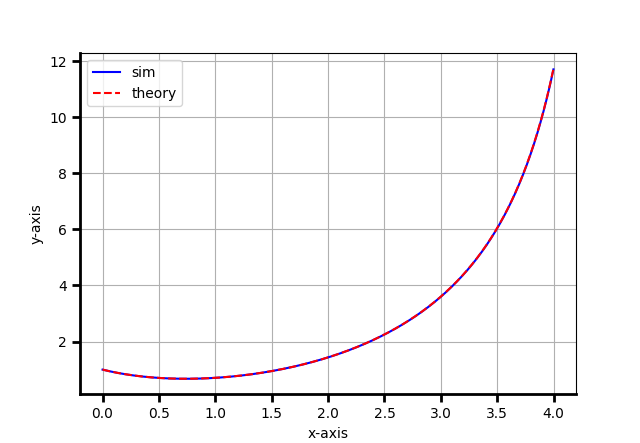
\includegraphics[width=\columnwidth]{fig/Figure_1.png}  
    \caption{Verification}
    \label{fig:example}  % Label for referencing
\end{figure}
\end{enumerate}
               
\end{document}

